\appendix
\section{Node Types for FlatZinc}\label{sec:node-types}
Table \ref{tab:nodes} shows all the node types used to decompose FlatZinc models to graphs. While this nodes have been especially designed around the FlatZinc interface, be believe that they could easily generalise to different languages with the only exception of global nodes which are tied to the one supported by the solver used for the MiniZinc to FlatZinc conversion (Gecode in our case).
\begin{table}
  \centering
  \resizebox{\textwidth}{!}{
    \begin{tabular}{|c|c|c|c|c|c|}
      \cline{0-5}
      Name & Type & Subtype & Is Cut & Is Global & Description \\
      \cline{0-5}
      Variable & variable & -- & No & No & Problem variable \\
      Parameter & parameter & -- & No & No & Literal value or parameter \\
      Multiply & operator & mul\_node & No & No & Multiplication operator \\
      Linear Sum & operator & lin\_sum\_node & Yes & No & Weighted sum of variables \\
      Sum & operator & sum\_node & No & No & Sum operator \\
      Equality & constraint & equality\_node & No & No & Equality constraint \\
      Inequality & constraint & inequality\_node & No & No & Equality constraint \\
      Less than & constraint & le\_node & No & No & Strictly less than constraint \\
      Less or Equal & constraint & leq\_node & No & No & Less than or equal constraint \\
      Imply & constraint & imply\_node & No & No & Logical implication \\
      If and only if & constraint & iff\_node & No & No & Logical equivalence \\
      Not & constraint & not\_node & No & No & Logical negation \\
      Or & constraint & or\_node & No & No & Logical disjunction \\
      And & constraint & and\_node & No & No & Logical conjunction \\
      Xor & constraint & xor\_node & No & No & Logical exclusive or \\
      Index & operator & index\_node & No & No & Array index operator \\
      Abs & operator & abs\_node & No & No & Absolute value operator \\
      Division & operator & division\_node & No & No & Integer division operator \\
      Max & operator & max\_node & No & No & Maximum operator \\
      Min & operator & min\_node & No & No & Minimum operator \\
      Modulo & operator & modulo\_node & No & No & Modulo operator \\
      Pow & operator & pow\_node & No & No & Power operator \\
      In & constraint & in\_node & No & No & Set membership constraint \\
      Card & operator & card\_node & No & No & Set cardinality operator \\
      Difference & operator & diff\_node & No & No & Set difference operator \\
      Intersect & operator & intersect\_node & No & No & Set intersection operator \\
      Subset & constraint & subset\_node & No & No & Set subset constraint \\
      Symmetric difference & operator & symdiff\_node & No & No & Set symmetric difference operator \\
      Union & operator & union\_node & No & No & Set union operator \\
      Maximise & solve & maximise\_node & No & No & Maximisation objective \\
      Minimise & solve & minimise\_node & No & No & Minimisation objective \\
      Array & operator & array\_node & No & No & Array container \\
      Cumulative & constraint & cumulative\_node & Yes & Yes & Global cumulative constraint \\
      Integer Element & operator & int\_element\_node & Yes & Yes & Global element constraint \\
      Linear equality iff & constraint & int\_lin\_eq\_impt\_node & Yes & No & Reified linear equality \\
      Array max & constraint & array\_int\_maximum\_node & Yes & Yes & Global array maximum constraint \\
      Schedule unary & constraint & schedule\_unary\_node & Yes & Yes & Global unary scheduling constraint \\
      Linear less than iff & constraint & int\_le\_imp\_node & Yes & No & Reified linear less than \\
      Maximum argument offset & constraint & maximum\_arg\_int\_offset\_node & Yes & Yes & Global maximum argument constraint \\
      Circuit & constraint & circuit\_node & Yes & Yes & Global circuit constraint \\
      Count equality & constraint & count\_eq\_node & Yes & Yes & Global count equality constraint \\
      Count equality iff & constraint & count\_eq\_reif\_node & Yes & Yes & Reified count equality constraint \\
      Set in iff & constraint & set\_in\_imp\_node & Yes & Yes & Reified set membership constraint \\
      Global cardinality & constraint & global\_cardinality\_node & Yes & Yes & Global cardinality constraint \\
      Global cardinality low up & constraint & global\_cardinality\_low\_up\_node & Yes & Yes & Global cardinality constraint with bounds \\
      Global cardinality low up closed & constraint & global\_cardinality\_low\_up\_closed\_node & Yes & Yes & Global cardinality constraint with closed bounds \\
      Xor iff & constraint & bool\_xor\_imp\_node & Yes & No & Reified exclusive or constraint \\
      No overlap & constraint & nooverlap\_node & Yes & Yes & Global no overlap constraint \\
      Regular & constraint & regular\_node & Yes & Yes & Global regular constraint \\
      All different & constraint & all\_different\_node & Yes & Yes & Global all different constraint \\
      Equality iff & constraint & eq\_imp\_node & Yes & Yes & Reified equality constraint \\
      All equal & constraint & all\_equal\_node & Yes & Yes & Global all equal constraint \\
      Boolean Element & operator & bool\_element\_node & Yes & No & Global element constraint (boolean) \\
      Array minimum & constraint & array\_int\_minimum\_node & Yes & No & Global array minimum constraint \\
      Bool clause iff & constraint & bool\_clause\_reif\_node & Yes & No & Reified boolean clause constraint \\
      Element 2d & operator & int\_element2d\_node & Yes & Yes & Global 2D element constraint \\
      Bin packing load & constraint & bin\_packing\_load\_node & Yes & Yes & Global bin packing load constraint \\
      Table & constraint & table\_int\_node & Yes & Yes & Global table constraint \\
      Precede & constraint & precede\_node & Yes & Yes & Global precede constraint \\
      Array less or equal & constraint & array\_int\_lq\_node & Yes & No & Global array less or equal constraint \\
      Linear less than iff & constraint & int\_lin\_le\_imp\_node & Yes & No & Reified linear less than \\
      Linear not equal iff & constraint & int\_lin\_ne\_imp\_node & Yes & No & Reified linear not equal \\
      Increasing integer & constraint & increasing\_int\_node (int) & Yes & Yes & Global increasing integer constraint \\
      Inverse & constraint & inverse\_offsets\_node & Yes & Yes & Global inverse constraint \\
      N value & constraint & nvalue\_node & Yes & Yes & Global n-value constraint \\
      Not equal iff & constraint & int\_ne\_imp\_node & Yes & No & Reified not equal constraint \\
      Increasing bool & constraint & increasing\_bool\_node & Yes & Yes & Global increasing boolean constraint \\
      Member integer & constraint & member\_int\_node & Yes & Yes & Global member integer constraint \\
      Table iff & constraint & table\_int\_imp\_node & Yes & Yes & Reified global table constraint \\
      At least & constraint & at\_least\_node & Yes & Yes & Global at least constraint \\
      At most & constraint & at\_most\_node & Yes & Yes & Global at most constraint \\
      Integer pow & constraint & int\_pow\_node & Yes & Yes & Global integer power constraint \\
      Global cardinality closed & constraint & global\_cardinality\_closed\_node & Yes & Yes & Global cardinality constraint closed \\
      \cline{0-5}
    \end{tabular}
  }
  \caption{Node types used in our graphs converted from FlatZinc.}
  \label{tab:nodes}
\end{table}

\section{On The Shallowness of the Graphs}\label{sec:graph-depth}
Figure \ref{fig:long-graph} shows the constraint that produces the deepest path currently implemented. A family of similar constraints are present and they usually differ from the type of constraint that replace the equality (e.g. inequality, less or equal than, etc.) The graph at this level has a diameter of 4 which is reduced to 2 when the cut is applied. Most supported constrains are, instead, quite simple with most of them having a diameter of one or two. For the full list of supported constraints we refer to the FlatZinc specification.\footnote{\url{https://docs.minizinc.dev/en/stable/lib-flatzinc.html}}

\begin{figure}[t]
  \centering
  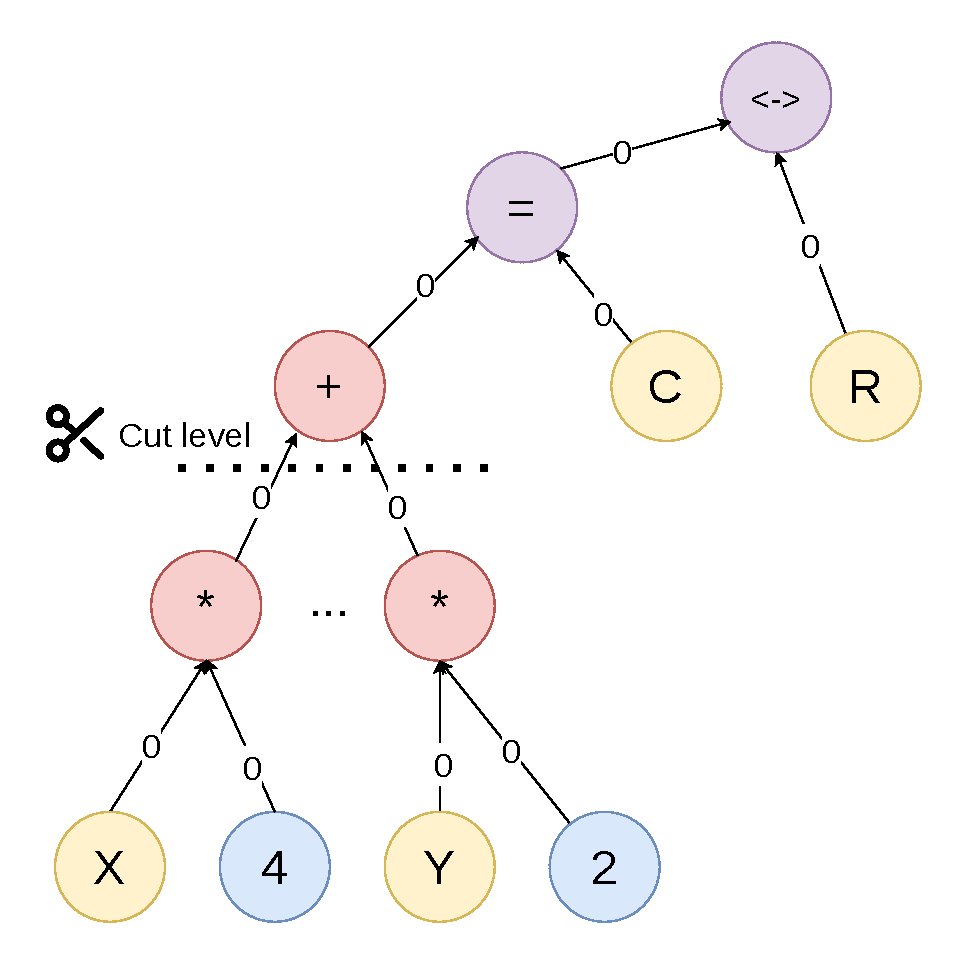
\includegraphics[width=.5\textwidth]{figures/long_graph.drawio}
  \caption{Representation of the deepest constraint currently present in the graph conversion. The constraint corresponds to $\sum_i var_i \times par_i = C \leftrightarrow R$. Variables are in yellow, parameters in blue, operators in red and constraints in purple.}
  \label{fig:long-graph}
\end{figure}

\section{All Borda Count Results}
Figures \ref{fig:RF-bordacount-all} and \ref{fig:nn-bordacount-all} show the results on the Borda count tasks for (respectively) RF and MLP classifiers trained with all Feature sets. RF results show similar results for all \texttt{WL} based features that include node information as well as \texttt{fzn2feat} features. On the other hand, MLP results show a trend similar to SVM where cut features significantly outperform the other \texttt{WL}-based features as well as showing an higher gap with respect to \texttt{fzn2feat}.

\begin{figure}
  \centering
  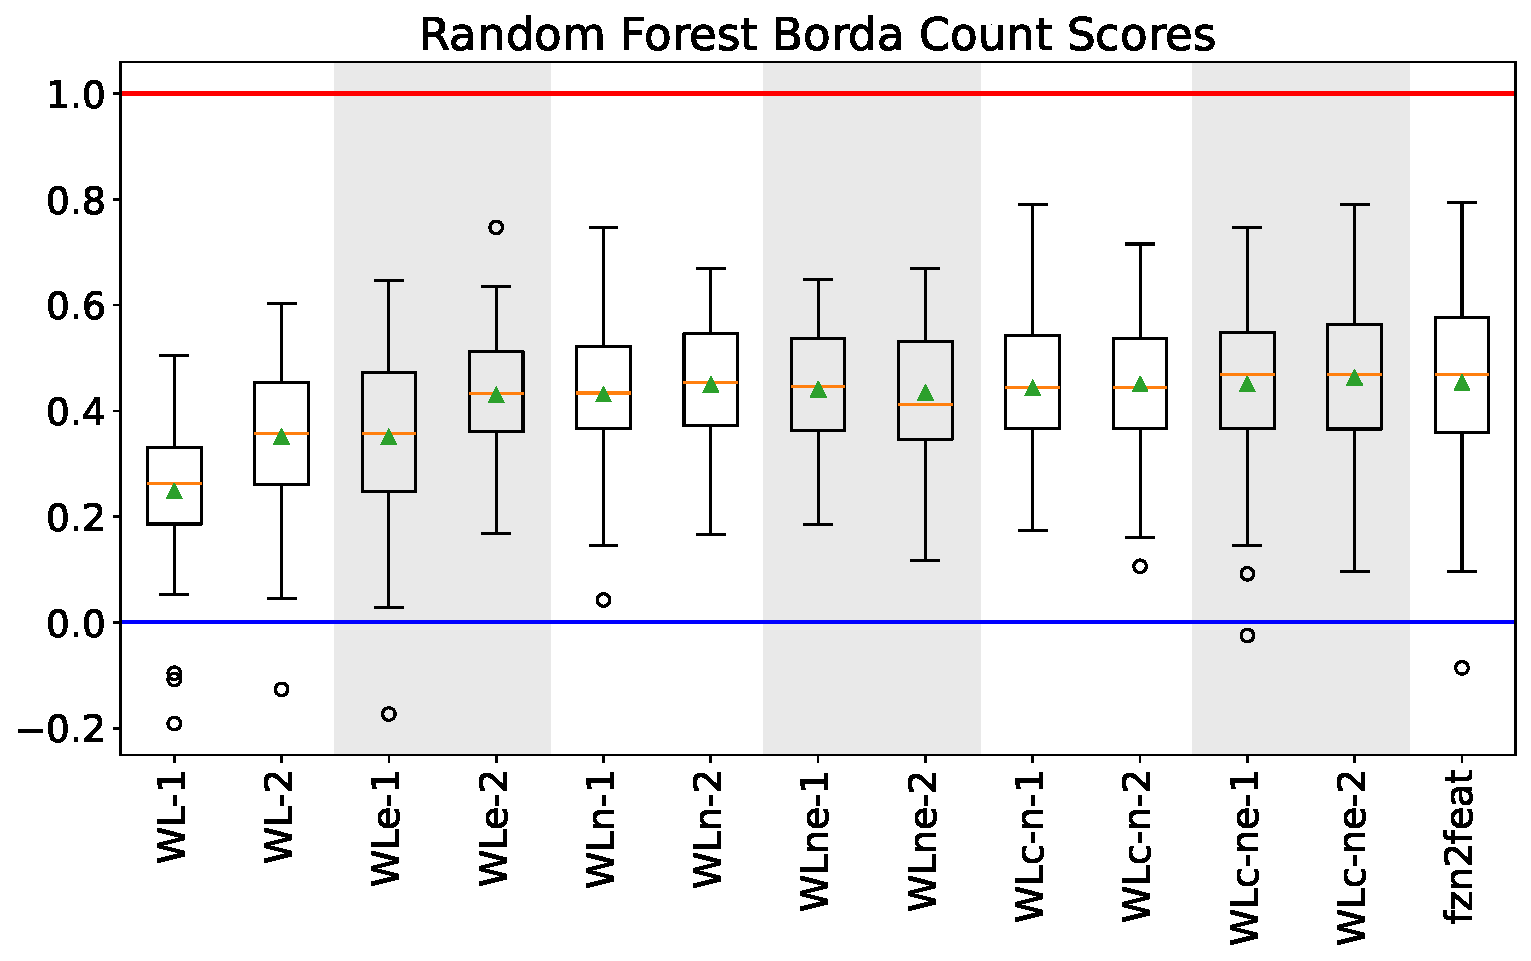
\includegraphics[width=.7\linewidth]{figures/all-wl-fzn2feat_score_forest}
  \caption{Results of all features sets trained with the RF classifier on the Borda count maximisation task.}
  \label{fig:RF-bordacount-all}
\end{figure}

\begin{figure}
  \centering
  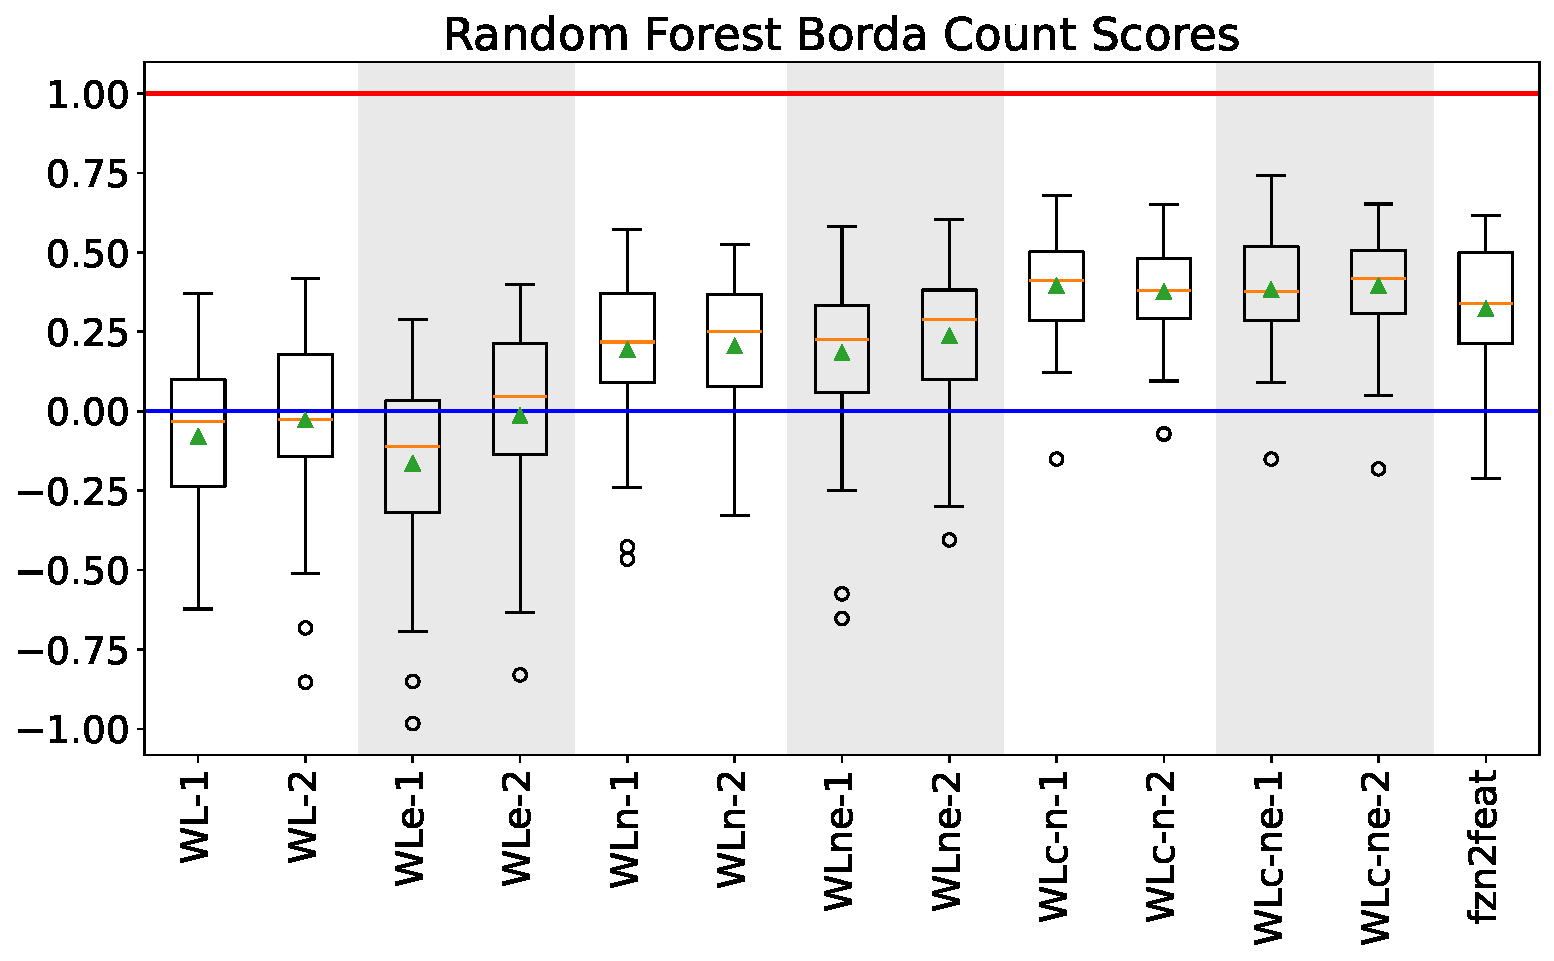
\includegraphics[width=.7\linewidth]{figures/all-wl-fzn2feat_score_nn}
  \caption{Results of all features sets trained with the MLP classifier on the Borda count maximisation task.}
  \label{fig:nn-bordacount-all}
\end{figure}

\section{All Algorithm Section Accuracy Results}
Figures \ref{fig:RF-acc-all} and \ref{fig:nn-acc-all} show the results on the Algorithm selection accuracy tasks for (respectively) RF and MLP classifiers trained with all Feature sets. Similarly to the Borda count counterpart, RF results show similar results for all \texttt{WL} based features that include node information as well as \texttt{fzn2feat} features, while, MLP results show a trend similar to SVM where cut features significantly outperform the other \texttt{WL}-based features as well as showing an higher gap with respect to \texttt{fzn2feat} (although less pronounced respect to the Borda Count).

\begin{figure}
  \centering
  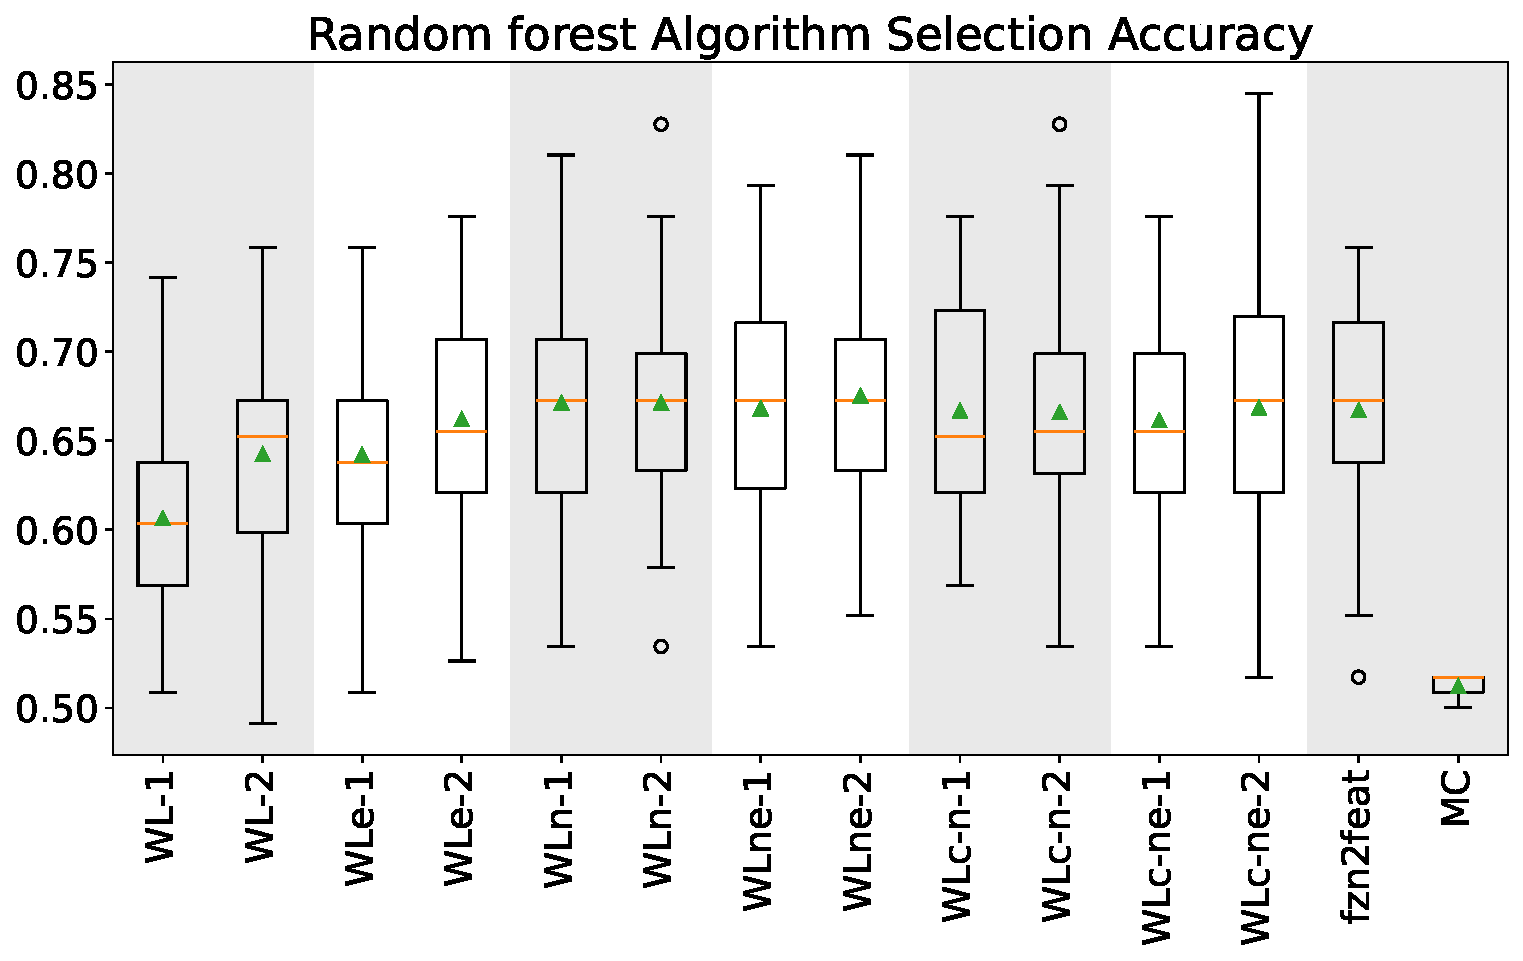
\includegraphics[width=.7\linewidth]{figures/all-wl-fzn2feat_accuracy_forest}
  \caption{Results of all features sets trained with the RF classifier on the Algorithm Selection accuracy maximisation task.}
  \label{fig:RF-acc-all}
\end{figure}

\begin{figure}
  \centering
  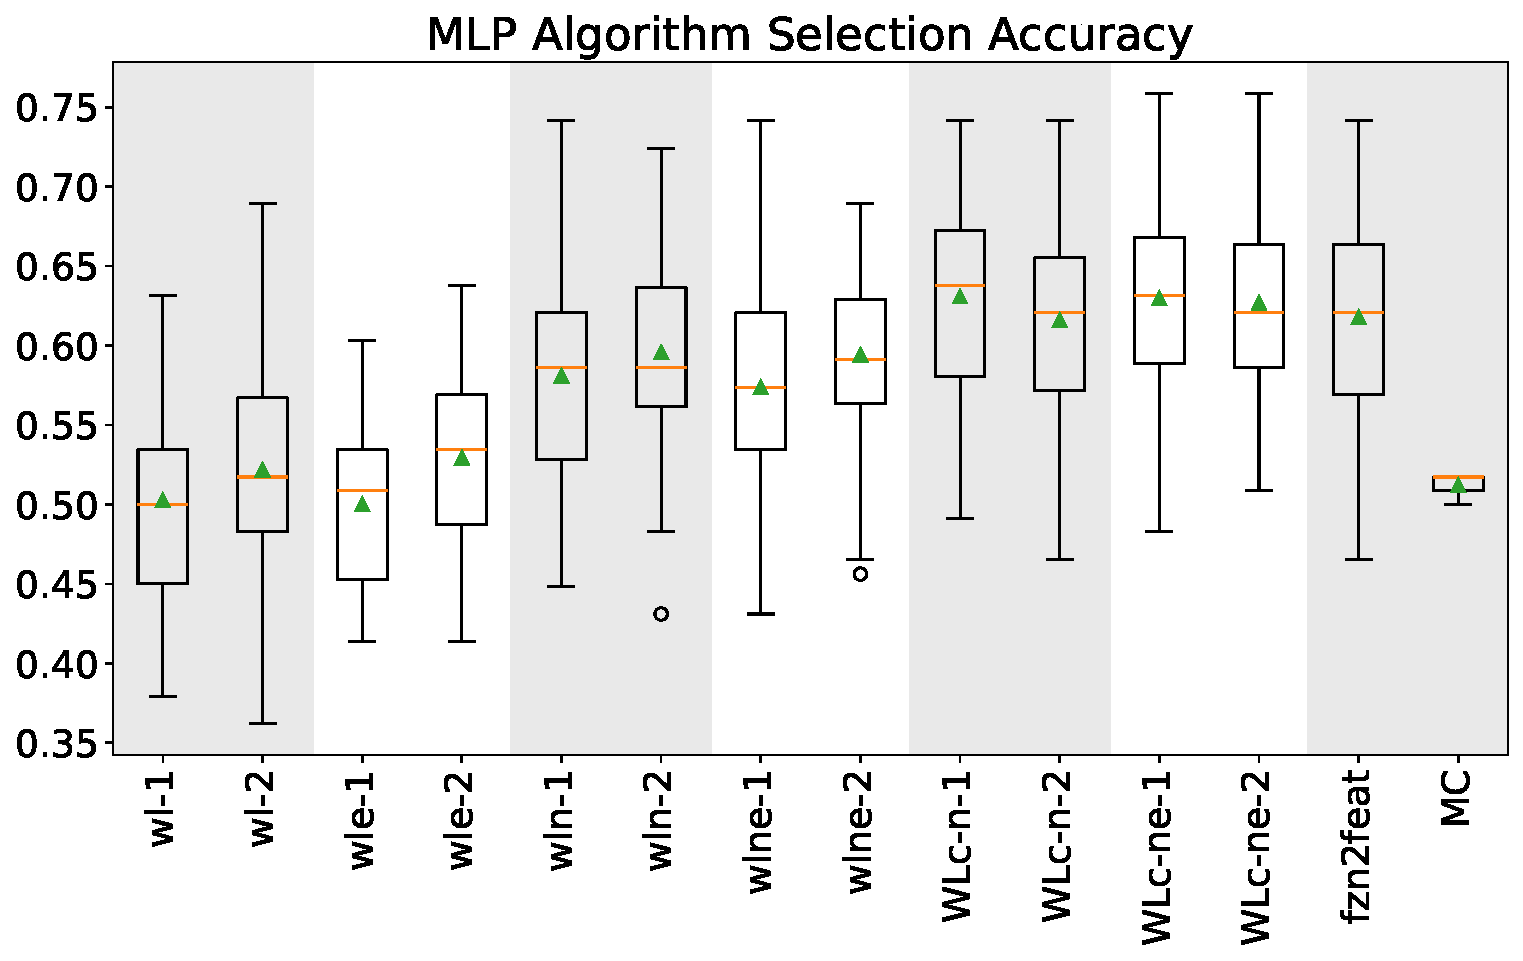
\includegraphics[width=.7\linewidth]{figures/all-wl-fzn2feat_accuracy_nn.pdf}
  \caption{Results of all features sets trained with the MLP classifier on the Algorithm Selection accuracy maximisation task.}
  \label{fig:nn-acc-all}
\end{figure}

\section{Ablation Study on the Importance of Concatenating All Aggregation Levels}\label{sec:ablation-study}
To asses whether only using the last aggregation level of the \texttt{WL} resulted or not in a loss of performance, we conducted an ablation study on the best performing features: \texttt{WLc-1/2}, \texttt{WLce-1/2}, \texttt{WLn-1/2}, and \texttt{WLne-1/2} across all different tasks and ML models. Results can be found in Tables \ref{tab:all-levels-borda} (Borda score), \ref{tab:all-levels-accuracy} (algorithm selection accuracy), and \ref{tab:all-levels-par} (parallel prediction). The tables show the mean and median results of the ML models trained on only the last level or on all levels of aggregation as well as the p value computed with the Wilcoxon test. In all cases but one, the results are not statistically significant. The only case in which they are (\texttt{WLc-1} in SVM algorithm selection accuracy prediction), it is in favour of the features with only the last aggregation level.

\begin{table}[t]
  \centering
  \begin{subtable}{.49\linewidth}
    \centering
    \caption{Results of SVM models.}
    \resizebox{\linewidth}{!}{
      \begin{tabular}{llllll}
        \toprule
        & Last mean & All-levels mean & Last median & All-levels median & p value \\
        \midrule
        \texttt{WLn-2} & 0.283 & 0.243 & 0.276 & 0.266 & 0.357 \\
        \texttt{WLne-2} & 0.276 & 0.236 & 0.275 & 0.266 & 0.201 \\
        \texttt{WLc-1} & 0.485 & 0.441 & 0.506 & 0.473 & 0.399 \\
        \texttt{WLn-1} & 0.210 & 0.196 & 0.245 & 0.237 & 0.632 \\
        \texttt{WLce-2} & 0.479 & 0.432 & 0.475 & 0.460 & 0.318 \\
        \texttt{WLce-1} & 0.470 & 0.440 & 0.513 & 0.487 & 0.681 \\
        \texttt{WLc-2} & 0.472 & 0.432 & 0.504 & 0.456 & 0.198 \\
        \texttt{WLne-1} & 0.226 & 0.212 & 0.258 & 0.245 & 0.561 \\
        \bottomrule
      \end{tabular}
    }
  \end{subtable}

  \vspace{1em} % Optional spacing between rows

  \begin{subtable}{.49\linewidth}
    \centering
    \caption{Results of RF models.}
    \resizebox{\linewidth}{!}{
      \begin{tabular}{llllll}
        \toprule
        & Last mean & All-levels mean & Last median & All-levels median & p value \\
        \midrule
        \texttt{WLne-2} & 0.433 & 0.475 & 0.412 & 0.488 & 0.114 \\
        \texttt{WLce-1} & 0.450 & 0.456 & 0.469 & 0.484 & 0.774 \\
        \texttt{WLne-1} & 0.440 & 0.452 & 0.447 & 0.455 & 0.509 \\
        \texttt{WLce-2} & 0.462 & 0.450 & 0.468 & 0.445 & 0.472 \\
        \texttt{WLn-1} & 0.431 & 0.464 & 0.434 & 0.486 & 0.318 \\
        \texttt{WLn-2} & 0.449 & 0.464 & 0.454 & 0.465 & 0.745 \\
        \texttt{WLc-1} & 0.443 & 0.460 & 0.444 & 0.465 & 0.608 \\
        \texttt{WLc-2} & 0.450 & 0.449 & 0.444 & 0.459 & 0.863 \\
        \bottomrule
      \end{tabular}
    }
  \end{subtable}
  \begin{subtable}{.49\linewidth}
    \centering
    \caption{Results of MLP models.}
    \resizebox{\linewidth}{!}{
      \begin{tabular}{llllll}
        \toprule
        & Last mean & All-levels mean & Last median & All-levels median & p value \\
        \midrule
        \texttt{WLc-2} & 0.393 & 0.406 & 0.410 & 0.433 & 0.415 \\
        \texttt{WLc-1} & 0.399 & 0.387 & 0.413 & 0.390 & 0.730 \\
        \bottomrule
      \end{tabular}
    }
  \end{subtable}
  \caption{Results of the ML models trained for Borda count maximisation on \texttt{WL} features with (all-levels) and without (last) all aggregation levels. Results report mean and median scores as well as the p value calculated with the Wilcoxon test.}
  \label{tab:all-levels-borda}
\end{table}

\begin{table}[t]
  \centering
  \begin{subtable}{.49\linewidth}
    \centering
    \caption{Results of SVM models.}
    \resizebox{\linewidth}{!}{
      \begin{tabular}{llllll}
        \toprule
        & Last mean & All-levels mean & Last median & All-levels median & p value \\
        \midrule
        \texttt{WLc-1} & 0.695 & 0.663 & 0.681 & 0.655 & 0.030 \\
        \texttt{WLc-2} & 0.687 & 0.664 & 0.690 & 0.672 & 0.089 \\
        \texttt{WLce-1} & 0.693 & 0.674 & 0.690 & 0.664 & 0.251 \\
        \texttt{WLce-2} & 0.690 & 0.659 & 0.690 & 0.661 & 0.060 \\
        \texttt{WLn-1} & 0.589 & 0.596 & 0.591 & 0.600 & 0.364 \\
        \texttt{WLn-2} & 0.607 & 0.591 & 0.603 & 0.603 & 0.217 \\
        \texttt{WLne-1} & 0.589 & 0.597 & 0.600 & 0.596 & 0.336 \\
        \texttt{WLne-2} & 0.605 & 0.604 & 0.603 & 0.603 & 0.974 \\
        \bottomrule
      \end{tabular}
    }
  \end{subtable}

  \vspace{1em} % Optional spacing between rows

  \begin{subtable}{.49\linewidth}
    \centering
    \caption{Results of RF models.}
    \resizebox{\linewidth}{!}{
      \begin{tabular}{llllll}
        \toprule
        & Last mean & All-levels mean & Last median & All-levels median & p value \\
        \midrule
        \texttt{WLc-1} & 0.666 & 0.669 & 0.652 & 0.655 & 0.615 \\
        \texttt{WLc-2} & 0.666 & 0.661 & 0.655 & 0.655 & 0.619 \\
        \texttt{WLce-1} & 0.661 & 0.665 & 0.655 & 0.661 & 0.930 \\
        \texttt{WLce-2} & 0.668 & 0.659 & 0.672 & 0.655 & 0.322 \\
        \texttt{WLn-1} & 0.671 & 0.678 & 0.672 & 0.672 & 0.584 \\
        \texttt{WLn-2} & 0.671 & 0.677 & 0.672 & 0.672 & 0.611 \\
        \texttt{WLne-1} & 0.668 & 0.674 & 0.672 & 0.672 & 0.804 \\
        \texttt{WLne-2} & 0.675 & 0.672 & 0.672 & 0.672 & 0.866 \\
        \bottomrule
      \end{tabular}
    }
  \end{subtable}
  \begin{subtable}{.49\linewidth}
    \centering
    \caption{Results of MLP models.}
    \resizebox{\linewidth}{!}{
      \begin{tabular}{llllll}
        \toprule
        & Last mean & All-levels mean & Last median & All-levels median & p value \\
        \midrule
        \texttt{WLc-1} & 0.629 & 0.620 & 0.621 & 0.621 & 0.526 \\
        \texttt{WLc-2} & 0.621 & 0.624 & 0.626 & 0.621 & 0.690 \\
        \texttt{WLce-1} & 0.613 & 0.614 & 0.621 & 0.621 & 0.964 \\
        \bottomrule
      \end{tabular}
    }
  \end{subtable}
  \caption{Results of the ML models trained for algorithm selection accuracy maximisation on \texttt{WL} features with (all-levels) and without (last) all aggregation levels. Results report mean and median scores as well as the p value calculated with the Wilcoxon test.}
  \label{tab:all-levels-accuracy}
\end{table}

\begin{table}[t]
  \centering
  \begin{subtable}{.49\linewidth}
    \centering
    \caption{Results of SVM models.}
    \resizebox{\linewidth}{!}{
      \begin{tabular}{llllll}
        \toprule
        & Last mean & All-levels mean & Last median & All-levels median & p value \\
        \midrule
        \texttt{WLc-1} & 0.622 & 0.620 & 0.633 & 0.617 & 0.935 \\
        \texttt{WLc-2} & 0.611 & 0.626 & 0.605 & 0.617 & 0.327 \\
        \texttt{WLce-1} & 0.618 & 0.627 & 0.633 & 0.622 & 0.295 \\
        \texttt{WLce-2} & 0.625 & 0.628 & 0.622 & 0.625 & 0.851 \\
        \texttt{WLn-1} & 0.625 & 0.619 & 0.617 & 0.633 & 0.615 \\
        \texttt{WLn-2} & 0.604 & 0.615 & 0.600 & 0.617 & 0.438 \\
        \texttt{WLne-1} & 0.633 & 0.610 & 0.627 & 0.617 & 0.095 \\
        \texttt{WLne-2} & 0.604 & 0.601 & 0.600 & 0.600 & 0.845 \\
        \bottomrule
      \end{tabular}
    }
  \end{subtable}

  \vspace{1em} % Optional spacing between rows

  \begin{subtable}{.49\linewidth}
    \centering
    \caption{Results of RF models.}
    \resizebox{\linewidth}{!}{
      \begin{tabular}{llllll}
        \toprule
        & Last mean & All-levels mean & Last median & All-levels median & p value \\
        \midrule
        \texttt{WLc-1} & 0.642 & 0.651 & 0.633 & 0.650 & 0.409 \\
        \texttt{WLc-2} & 0.634 & 0.638 & 0.650 & 0.650 & 0.658 \\
        \texttt{WLce-2} & 0.643 & 0.649 & 0.633 & 0.661 & 0.619 \\
        \texttt{WLce-1} & 0.654 & 0.645 & 0.650 & 0.633 & 0.435 \\
        \texttt{WLn-1} & 0.635 & 0.645 & 0.650 & 0.650 & 0.369 \\
        \texttt{WLn-2} & 0.645 & 0.650 & 0.644 & 0.650 & 0.476 \\
        \texttt{WLne-1} & 0.643 & 0.634 & 0.647 & 0.633 & 0.464 \\
        \texttt{WLne-2} & 0.642 & 0.648 & 0.650 & 0.650 & 0.631 \\
        \bottomrule
      \end{tabular}
    }
  \end{subtable}
  \begin{subtable}{.49\linewidth}
    \centering
    \caption{Results of MLP models.}
    \resizebox{\linewidth}{!}{
      \begin{tabular}{llllll}
        \toprule
        & Last mean & All-levels mean & Last median & All-levels median & p value \\
        \midrule
        \texttt{WLc-2} & 0.652 & 0.649 & 0.650 & 0.650 & 0.984 \\
        \texttt{WLc-1} & 0.647 & 0.650 & 0.633 & 0.650 & 0.891 \\
        \bottomrule
      \end{tabular}
    }
  \end{subtable}
  \caption{Results of the ML models trained for parallel prediction on \texttt{WL} features with (all-levels) and without (last) all aggregation levels. Results report mean and median scores as well as the p value calculated with the Wilcoxon test.}
  \label{tab:all-levels-par}
\end{table}